% ### Uses XeLaTeX ### %
% ### Needs beamer-master ### %
\documentclass[aspectratio=169]{beamer} %. Aspect Ratio 16:9
\usetheme{AI2} % beamerthemeSprace.sty
% DATA FOR FOOTER
\date{2020}
\title{Deep Learning HPC}
\author{}
\institute{Advanced Institute for Artificial Intelligence (AI2)}
\begin{document}
% ####################################
% FIRST SLIDE 						:: \SliTit{This is the Title of the Talk}{A. B. Name}{Sprace}
% SUB-TITLE SLIDE 					:: \SliSubTit{<title>}{<explanation}
% SUB-SUB-TITLE SLIDE				:: \SliSubSubTit{<title>}{<explanation}
% SLIDE WITH TITLE 					:: \SliT{Title}{Content}
% SLIDE NO TITLE 						:: \Sli{Content} 
% SLIDE DOUBLE COLUMN WITH TITLE 	:: \SliDT{Title}{First Column}{Second Column}
% SLIDE DOUBLE COLUMN NO TITLE 		:: \SliD{First Column}{Second Column}
% SLIDE ADVANCED WITH TITLE 			:: \SliAdvT{Title}{Content}
% SLIDE ADVANCED NO TITLE 			:: \SliAdv{Content}
% SLIDE ADVANCED DOUBLE WITH TITLE 	:: \SliAdvDT{Title}{First Column}{Second Column}
% SLIDE ADVANCED DOUBLE NO TITLE 	:: \SliAdvD{First Column}{Second Column}
% SLIDE BLACK						:: \Black{ <Content> }
% SLIDE WHITE						:: \White{ <Content> }
% ITEMIZATION 						:: \begin{itemize}  \iOn{First} \iTw {Second} \iTh{Third} \end{itemize}
% COMMENT TEXT				 		:: \note{<comment>}
% SECTION 							:: \secx{Section} | \secxx{Sub-Section}
% BOLD SPRACE COLOR				:: \bfs{<text>}
% TABLE OF CONTENT					:: \tocitem{<title>}{<content>}
% LEFT ALIGN EQUATION				:: \begin{flalign*}  & <equation> &   \end{flalign*}
% CENTER ALIGN EQUATION	S			:: \begin{gather*} <equations>  \end{gather*}
% SLASH								:: \slashed{<>}
% BAR								:: \barr{<letter>} instead of \bar{<letter>}
% THEREFORE						:: use \portanto (larger and bold}
% 2 or 3 MATH SYMBOLS				:: \overset{<up>}{<down>} &  \underset{<below>}{\overset{<above>}{<middle>}}  
% INSERT TEXT IN FORMULA			:: \ins{<text>}
% EXERCISE							:: \exe{<exercise #>}{<exercise text>}
% SUGGESTED READING BOX			:: \sug{<references>}
% CITATION							:: \cittex{<citation>}
% CITATION DOUBLE COLUMN 			:: \cittexD{<citation>}
% TEXT POSITION						:: \texpos{<Xcm>}{<Ycm>}{<text>} origin = center of slide : x right | y down
% REFERENCE AT BOTTOM  S/D SLIDE		:: \refbotS{<reference>} \refbotD{<reference>}
% HIDDEN SLIDE						:: \hid
% COLOR BOX 						:: \blu{blue} + \red{rec} + \yel{yellow} + \gre{green} + \bege{beige}
% FRAME 							:: \fra{sprace} \frab{blue} \frar{red} + \fray{yellow} + \frag{green}		
% FIGURE 							:: \img{X}{Y}{<scale>}{Figure.png} 
% FIGURE							:: \includegraphics[scale=<scale>]{Figures/.png}
% FIGURE DOUBLE SLIDE NO TITLE		::  \img{-4}{0.5}{<scale>}{Figure.png} % Image 1st half
%									::  \img{4}{0.5}{<scale>}{Figure.png} % Image 2nd half
% FIGURE DOUBLE SLIDE WITH TITLE		::  \img{-4}{0}{<scale>}{Figure.png} % Image 1st half
%									::  \img{4}{0}{<scale>}{Figure.png} % Image 2nd half
% INCLUDING SWF (Flash)				:: \usepackage{media9} and \includemedia >> USE ACROBAT <<
%%%%%%%%%%%%%%%%%%%%%%%%%%%%%%%%%%%%%%%%%%%%%%%%%%
% ###############################################################################
% FIRST SLIDE
\SliTit{Deep Learning HPC}{Advanced Institute for Artificial Intelligence -- AI2}{https://advancedinstitute.ai}


% SLIDE ADVANCED  WITH TITLE
\SliAdvT{Deep Learning HPC}{ 

Agenda

\begin{itemize}
  \iOn{HPC}
  \iOn{GPU}
  \iOn{Tensorflow}
  \iOn{Conteiner}
\end{itemize}

}

\SliAdvT{Introdução a HPC}{ 

O que é Computação de alto Desempenho ou HPC (High Performance Computing)?

\begin{itemize}
  \iOn{É uma área de pesquisa que lida com desafios relacionados com execução de aplicações com alto custo computacional}
  
    \iTw{Normalmente, tais aplicações são utilizadas com muita frequência, e qualquer melhoria de desempenho provocam impacto}
    
  \iOn{Avanço no desenvolvimento de arquiteturas computacionais com maior poder computacional}
  
      \iTw{Uma arquitetura computacional mais moderna provê recursos para melhorar o desempenho, porém a utilização de tais recursos nem sempre é trivial}

\end{itemize}
}


\SliAdvT{Introdução a HPC}{ 

Otimização de desempenho de aplicações

\begin{itemize}

 \iOn{Caracterização das demandas computacionais das aplicações, por exemplo, demanda por espaço de armazenamento, processamento, memória RAM, etc}

\iOn{Segmentação da aplicação em parte menores para que sejam executadas simultaneamente em diferentes recursos de uma arquitetura (paralelismo)}

\iOn{Desenvolvimento de camadas de software otimizadas para diversas arquiteturas computacionais}
\iTw{Tais camadas abstraem a complexidade do trabalho de otimização e permitem uso eficiente da arquitetura}

\end{itemize}
}

 \SliAdvT{Introdução a HPC}{ 

Impacto no tempo de resposta no uso de aplicações com alto custo computacional

\begin{itemize}
 
 \iOn{Aplicações de Aprendizagem Profunda (Deep Learning) normalmente são computacionalmente intensivas}
 
 \iTw{Busca por hiperparâmetros}
 \iTw{Treino do modelo com novos conjuntos de dados}
 \iTw{Prototipação de modelos}
 
 \iOn{Quanto mais rápido uma aplicação de aprendizagem profunda é executada, ainda que com um ganho não tão expressivo, apresenta impacto alto no trabalho dos especialistas desse domínio}
 

\end{itemize}
}

\SliAdvT{Introdução a HPC}{ 

Arquitetura uniprocessador

\begin{itemize}
  \iOn{Novas gerações de processadores aumentaram o desempenho (Lei de Moore)}
  \iTw{Até o desempenho do processador atingir seu limite}
  \iOn{Tendências para aumento de desempenho}
        \iTw{Mais unidades de processamento em um único processador}
        \iTw{Mais processadores na mesma máquina}
  \iOn{Para obter melhor desempenho, os desenvolvedores DEVEM explorar o paralelismo.}
\end{itemize}

}

\SliAdvT{Introdução a HPC}{ 

\begin{itemize}
  \iOn{Um computador paralelo é um sistema de computador que usa vários elementos de processamento simultaneamente de maneira cooperativa para resolver um problema computacional}

  \iOn{O processamento paralelo inclui técnicas e tecnologias que permitem calcular em paralelo}

  \iTw{Hardware, redes, sistemas operacionais, bibliotecas paralelas, linguagens, compiladores, algoritmos, ferramentas,…}

  \iOn{O paralelismo é natural}

    \iTw{Problemas de computação diferem em nível / tipo de paralelismo}

\end{itemize}

}

\SliAdvT{Introdução a HPC}{ 

Modelo de desempenho em processadores atuais

\begin{itemize}
\iOn{Processador e sistema de memória trabalham de forma independente}
\iOn{O desempenho da arquitetura computacional é medido de forma complementar}

\iTw{O desempenho do processador depende da eficiencia do sistema de memória entregar os dados para os registradores do processador}

\iTh{Se os dados são entregues de modo ineficiente, o processoador pode ficar ocioso em muitos momentos}

\iTw{O sistema de memória trabalha de modo eficiente se a vazão do processador é alta}
\iTh{Se o processoador não executa as operações de modo eficiente, o sistema de memória pode ficar ocioso em muits momentos}

\end{itemize}

}

\SliAdvT{Introdução a HPC}{ 

Técnicas para otimização de Desempenho

\begin{itemize}
    \iOn{Processador}
    \iTw{Vetorização permite executar uma mesma intrução para conjuntos diferentes de dados}
    
    \iOn{Sistema de memória}
    \iTw{Múltiplos níveis de memória permitem antecipar o envio de dados para o processador, aumentando a eficiência da execução das instruções}
\end{itemize}

}

\SliAdvT{Introdução a HPC}{ 

\begin{center}
    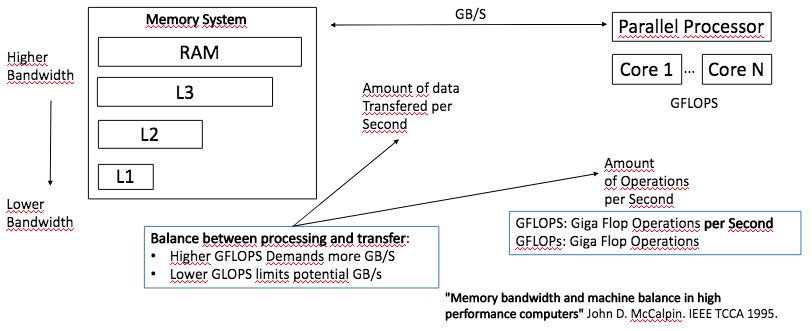
\includegraphics[scale=0.50]{performance-model.png}     
\end{center}

}
    
\SliAdvT{Introdução a HPC}{ 
As arquiteturas computacionais atuais, podem também ser compostas por coprocessadores ou aceleradores

\begin{center}
    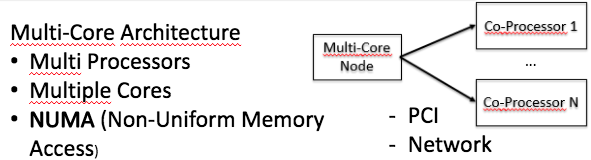
\includegraphics[scale=0.65]{no-heterogeneo.png}     
\end{center}
}

\SliAdvT{Introdução a HPC}{ 
%\tikz[parallelism.png, overlay] \node[anchor=center] at ($(current page.center)+(0,0)$) {(0,0)};
Uma forma de montar uma arquitetura computacional paralela é unificar diversos processador idênticos

\begin{center}
    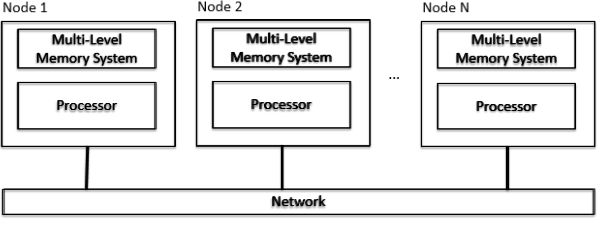
\includegraphics[scale=0.60]{homogeneo.png}     
\end{center}
}

\SliAdvT{Paralelismo}{ 
Outra forma de montar uma arquitetura computacional paralela é unificar diversos processador que podem ser diferentes entre si (Arquiteturas Heterogêneas)
\begin{center}
    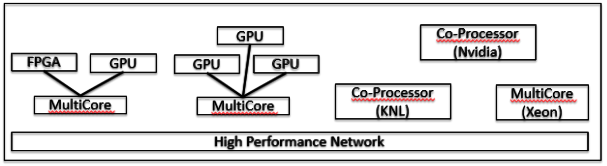
\includegraphics[scale=0.70]{heterogeneidade.png}     
\end{center}
}

\SliAdvT{Níveis de paralelismo}{ 

\begin{itemize}
  \iOn{Paralelismo no nível de instrução}
  \iTw{Mecanismos do processador para aumentar o desempenho }
  \iOn{Paralelismo no nível de dados(Vetorização)}
  \iTw{Execucao de mais de instrução identicas em paralelo para conjuntos distintos de dados, utilizando registradores vetoriais do processador} 
  \iTw{Vetorização em geral é combinada com técnicas de acesso eficiente utilizando múltiplos níveis de memória (cache)}
  
\end{itemize}

}

\SliAdvT{Níveis de paralelismo}{ 

\begin{itemize}
  \iOn{Paralelismo no nível de tarefa (Thread) OpenMP}
  \iTw{Múltiplas threads sendo executadas em paralelo}
  \iOn{Paralelismo no nível de processo}
  \iTw{Mesmo programa em diferentes computadores coordenado a execução por troca de mensagens pela rede (MPI)}
  \iOn{offload}
  \iTw{Dividindo o processamento entre o processador e um ou mais co-processadores, como GPU por exemplo}

\end{itemize}

}

\SliAdvT{Paralelismo}{ 

Os níveis de paralelismos podem ser usados de modo combinado por uma única aplicação

\begin{center}
    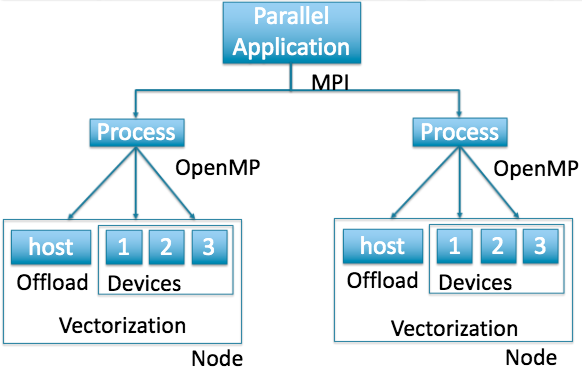
\includegraphics[scale=0.60]{NIVEIS-COMBINADOS.png}     
\end{center}
}

\SliAdvT{Paralelismo}{ 

\begin{itemize}
  \iOn{Para utilizar arquiteturas paralelas é necessário dividir a aplicação em tarefas independentes}
  
  \iTw{As tarefas podem ser simultâneas e podem ser executadas ao mesmo tempo (execução paralela)}

  \iOn{As tarefas podem possuir algum nível de dependência, de tal forma que, uma tarefa pode necessitar de dados produzidos por outra tarefa antes de entrar em execução} 
  
  \iTw{Alguma forma de sincronização deve ser usada para impor (satisfazer) dependências}
  \iOn{No nível do software a paralelização deve considerar as sincronizações entre as tarefas}
\iOn{Quanto ao uso do hardware é necessário traçar estratégias para utilizar de modo eficiente cada recurso de otimização de desempenho}
\end{itemize}

}

\SliAdvT{Paralelismo}{ 

\begin{center}
    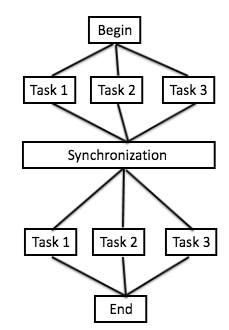
\includegraphics[scale=0.60]{parallelism.png}     
\end{center}
}

% SLIDE ADVANCED  WITH TITLE
\SliAdvT{GPU}{ 

GPU

\begin{itemize}
  \iOn{É um multiprocessador paralelo / multithread otimizado para processamento de imagem.}

\iTw{O processamento gráfico é uma aplicação massivamente paralela}


\iOn{GPGPU}

\iTw{Computação de uso geral usando GPU}

\iOn{A GPU serve como um processador gráfico programável e como uma plataforma de computação paralela escalável.}

\iTw{Os sistemas podem combinar CPU + GPU para executar aplicativos}
\end{itemize}
}

\SliAdvT{GPU}{ 

\begin{center}
    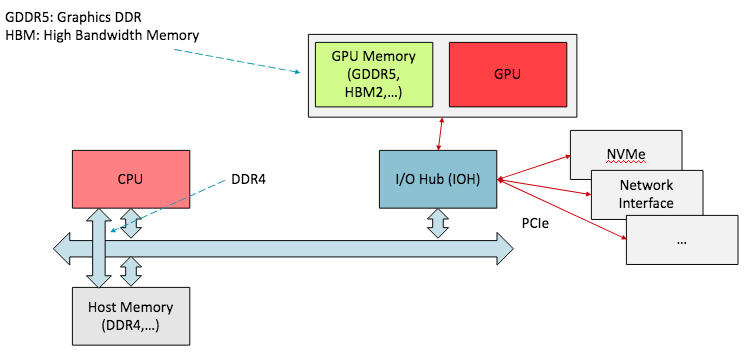
\includegraphics[scale=0.50]{gpu-arch.png}     
\end{center}
}

\SliAdvT{GPU}{ 

\begin{center}
    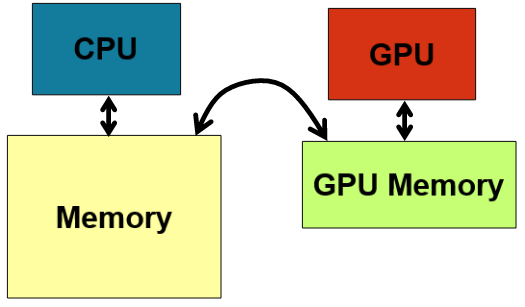
\includegraphics[scale=0.60]{gpu-arch2.png}     
\end{center}
}
\SliAdvT{GPU}{ 

\begin{center}
    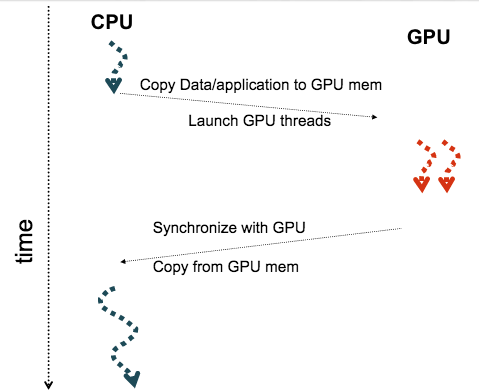
\includegraphics[scale=0.50]{gpu-arch3.png}     
\end{center}
}
\SliAdvT{GPU}{ 

\begin{center}
    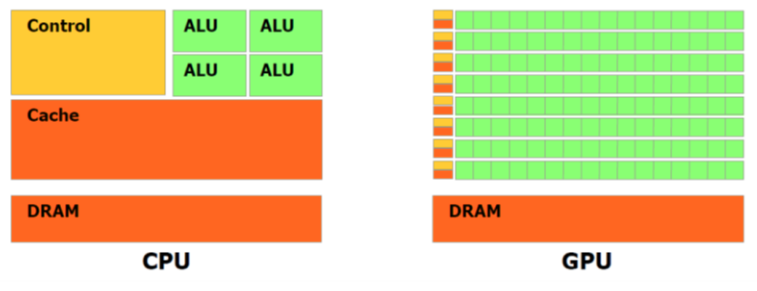
\includegraphics[scale=0.50]{gpu-arch4.png}     
\end{center}
}
\SliAdvT{GPU}{ 
\begin{itemize}
  \iOn{lógica simplificada (sem execução fora de ordem, sem previsão de ramificação) significa que muito mais do chip é dedicado à computação de ponto flutuante}

\iTw{Núcleo da CPU Core x Núcleo da GPU}

\iOn{Organizados como várias unidades, com cada unidade sendo efetivamente uma unidade vetorial, todos os núcleos fazendo a mesma coisa ao mesmo tempo}

\iTw{Kernel: uma rotina paralela para executar no hardware paralelo}

\iOn{Maior largura de banda de memória que a CPU}
\end{itemize}
}

\SliAdvT{GPU}{ 
\begin{itemize}
\iOn{Objetivo não geral}

\iTw{Aplicações massivamente paralelas}

\iTh{Processamento gráfico}

\iTw{Aplicativos que exploram a localidade da memória}

\iTh{Cada unidade paralela realiza acesso ao seu próprio subconjunto de dados}

\iTh{Os algoritmos de paralelo de dados utilizam atributos da GPU}

\iOn{Grandes matrizes de dados, taxa de transferência de streaming}

\iOn{Cálculo de ponto flutuante de baixa latência (FP)}
\end{itemize}
}

\SliAdvT{GPU}{ 

\begin{center}
    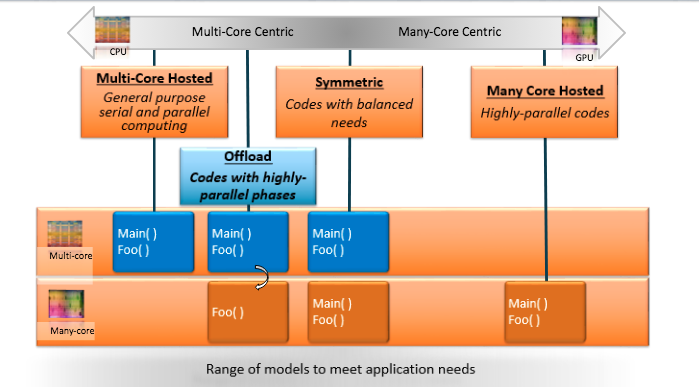
\includegraphics[scale=0.60]{offload.png}     
\end{center}
}

\SliAdvT{GPU}{ 
\begin{itemize}
  \iOn{Como usar os recursos da GPU}
  \iTw{Bibliotecas}
  \iTh{Cublas}
  \iTh{Tensorflow}
  \iTw{Extensões da linguagem (diretivas)}
  \iTh{OpenMP, OpenACC, OpenCL}
  \iTw{fácil de otimizar código}
  \iTw{Flexibilidade mínima}
  \iOn{Linguagem de Programação}
  \iTw{API Cuda}
  \iTw{Flexibilidade máxima}
  \iTw{Acesso de baixo nível}
\end{itemize}
}

\SliAdvT{GPU}{ 
Bibliotecas para Deep Learning
\begin{itemize}
  \iOn{Tensorflow}
  \iOn{Keras}
  \iOn{Caffe2}
  \iOn{Rapids}
\end{itemize}
}

\SliAdvT{Tensorflow}{ 
\begin{itemize}
  \iOn{Biblioteca de software de código aberto para computação numérica baseada no paradigma dataflow}

  \iOn{Execução de código otimizada porém acessível via API em um programa Python} 
  
  \iOn{Portabilidade: distribui a computação em uma ou mais CPUs ou GPUs em um nó}

\end{itemize}
}

\SliAdvT{Paradigma Dataflow}{ 
\begin{center}
    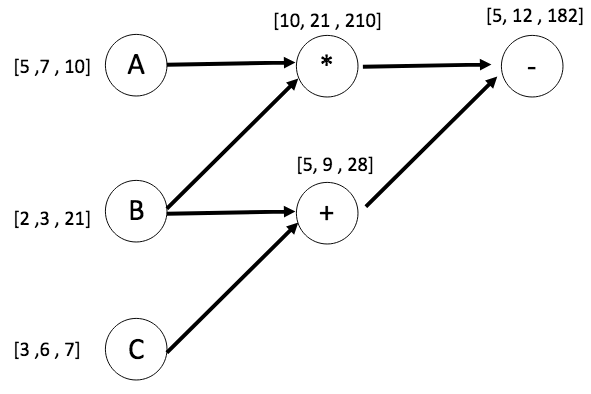
\includegraphics[scale=0.50]{DF.png} 
\end{center}
 
    
}

\SliAdvT{Montagem de Sistema}{

\begin{itemize}
\iOn{Um grande desafio em colocar aplicações em produção é montar o ambiente adequado de Sistema opearacional, versões de bibliotecas e parametrizações do sistema.}

\iOn{Quando há duas ou mais aplicações para colocar em produção o problema se torna ainda maior, pois um único ambiente deve atender duas demandas potencialmente distintas de sistema operacional}

\iOn{Uma solução para esse problema é a virtualização, que refere-se a mecanismo de criar uma visão do sistema operacional para cada aplicação}

\end{itemize}
}

\SliAdvT{Virtualização}{

\begin{itemize}
\iOn{Um mecanismo de virtualização muito simples são as maquinas virtuais}
\iOn{Outro mecanismo mais simples os ambientes virtuais como o conda}
\iOn{Duas desvantagens desses dois métodos:}
\iTw{Máquinas virtuais prejudicam o desempenho das aplicações}
\iTw{Ambientes virtuais são desprovidos de flexibilidade quanto a configuração do sistema operacional}

\end{itemize}
}

\SliAdvT{Linux Containers (LXC)}{ 

\begin{itemize}
\iOn{ Sistemas operacionais modernos oferecem recursos de virtualização no nível do sistema operacional}

\iOn{Tal virtualização  (chamadas conteineres) parte da premissa de que o kernel do SO permite a existência de múltiplas instâncias isoladas do espaço do usuário}

\iOn{Tais instâncias permitem criar um ambiente de SO próprio que acessa os recursos do computador e do SO instalado na máquina}

\iOn{Do ponto de vista dos programas em execução neles, parecem computadores reais }

\iOn{Conteineres são mais rápidos de iniciar, produzem pouca sobrecarga no desempenho da aplicação e são muito flexíveis quanto a montagem do Sistema operacional}

\end{itemize}
}


% SLIDE ADVANCED  WITH TITLE
\SliAdvT{Docker}{ 
\begin{itemize}

\iOn{ Docker é uma ferramenta para facilitar o processo de criação de containeres}

\iOn{ A plataforma docker-hub \footnote{https://hub.docker.com/} permite que usuários criem conteineres e compartilhem com outros usuários}
\iTw{Os comandos para gerenciar versões de conteineres docker é similar aos comandos do git hub}
\iOn{Um conteiner pode ser compartilhado e novos containeres podem ser criadas a partir de um conteiner existente}

\end{itemize}
}

\SliAdvT{Docker}{ 

Obter, rodar e terminar a execução de um conteiner

\begin{itemize}
  \iOn{Obter uma imagem (docker pull)}
  \iTw{docker pull bulletinboard:1.0}
  \iTw{Esse comando realiza o download da imagem do docker hub e controla a versão em uma pasta controlada pelo docker}
  \iOn{Rodar imagem (docker container run)}
  \iTw{docker container run --name bb bulletinboard:1.0}
  \iOn{Terminar a execução de um conteiner}
  \iTw{docker container rm --force bb}
\end{itemize}

}

\SliAdvT{Docker}{ 

Criando novos conteineres docker

\begin{itemize}
  \iOn{ Todo conteiner é definido por meio de um arquivo descritor chamado Dockerfile}

  \iOn{A partir de um descritor dockerfile é possível criar um conteiner}
  \iTw{docker image build -t bulletinboard:1.0 .}

  \iOn{Para armazenar um novo conteiner que teve seu descritor alterado pode-se utilizar a opção tag}
  \iTw{ image tag bulletinboard:1.0 silviostanzani/bulletinboard:1.0}
  \iOn{Para efetivamente armazenar uma versão local do conteiner no docker hub deve-se utilizar push }
  \iTw{ docker image push silviostanzani/bulletinboard:1.0}
\end{itemize}

}


\SliAdvT{Docker}{ 
Demonstração de uso de um container

\begin{itemize}
      \iOn{Criar uma imagem com streamlit e rede neural em Keras}
      \iOn{Armazenar no docker hub}
      \iOn{Recuperar e executar a imagem}
 \end{itemize}
}


\end{document}
